% Phụ lục W — hai lược đồ tuần tự còn lại (mục 5.3.3); hình sinh từ tools/diagrams/gen_sequence.py.

\section*{Phụ lục W. Lược đồ tuần tự chi tiết}
\label{apdx:tuantu}
\addcontentsline{toc}{section}{Phụ lục W. Lược đồ tuần tự chi tiết}

Hai lược đồ dưới đây bổ sung cho mục~\ref{subsec:tuantu}, cùng ký hiệu với Hình~\ref{fig:seq-dat-hang}. Hình~\ref{fig:seq-duyet-lo} theo một lô từ lúc nhà cung cấp tạo tới khi được duyệt và có mã QR: kiểm duyệt viên thao tác qua mô-đun vận hành, mô-đun vận hành gọi mô-đun sản phẩm, lô; phần mở dòng tồn, báo nhà cung cấp và tính lại vector đều chạy theo sự kiện \texttt{BatchApproved}, \texttt{ProductChanged}. Hình~\ref{fig:seq-danh-gia} theo một đánh giá: mô-đun đánh giá hỏi mô-đun bán lẻ để chắc chắn người gửi đã mua và đơn đã hoàn tất, chạy luật ngưỡng, rồi hoặc công khai ngay, hoặc chuyển cho kiểm duyệt viên quyết định.

\begin{figure}[p]
\centering
\begin{adjustbox}{max totalsize={\textwidth}{\dimexpr\textheight-1.6cm\relax},center}
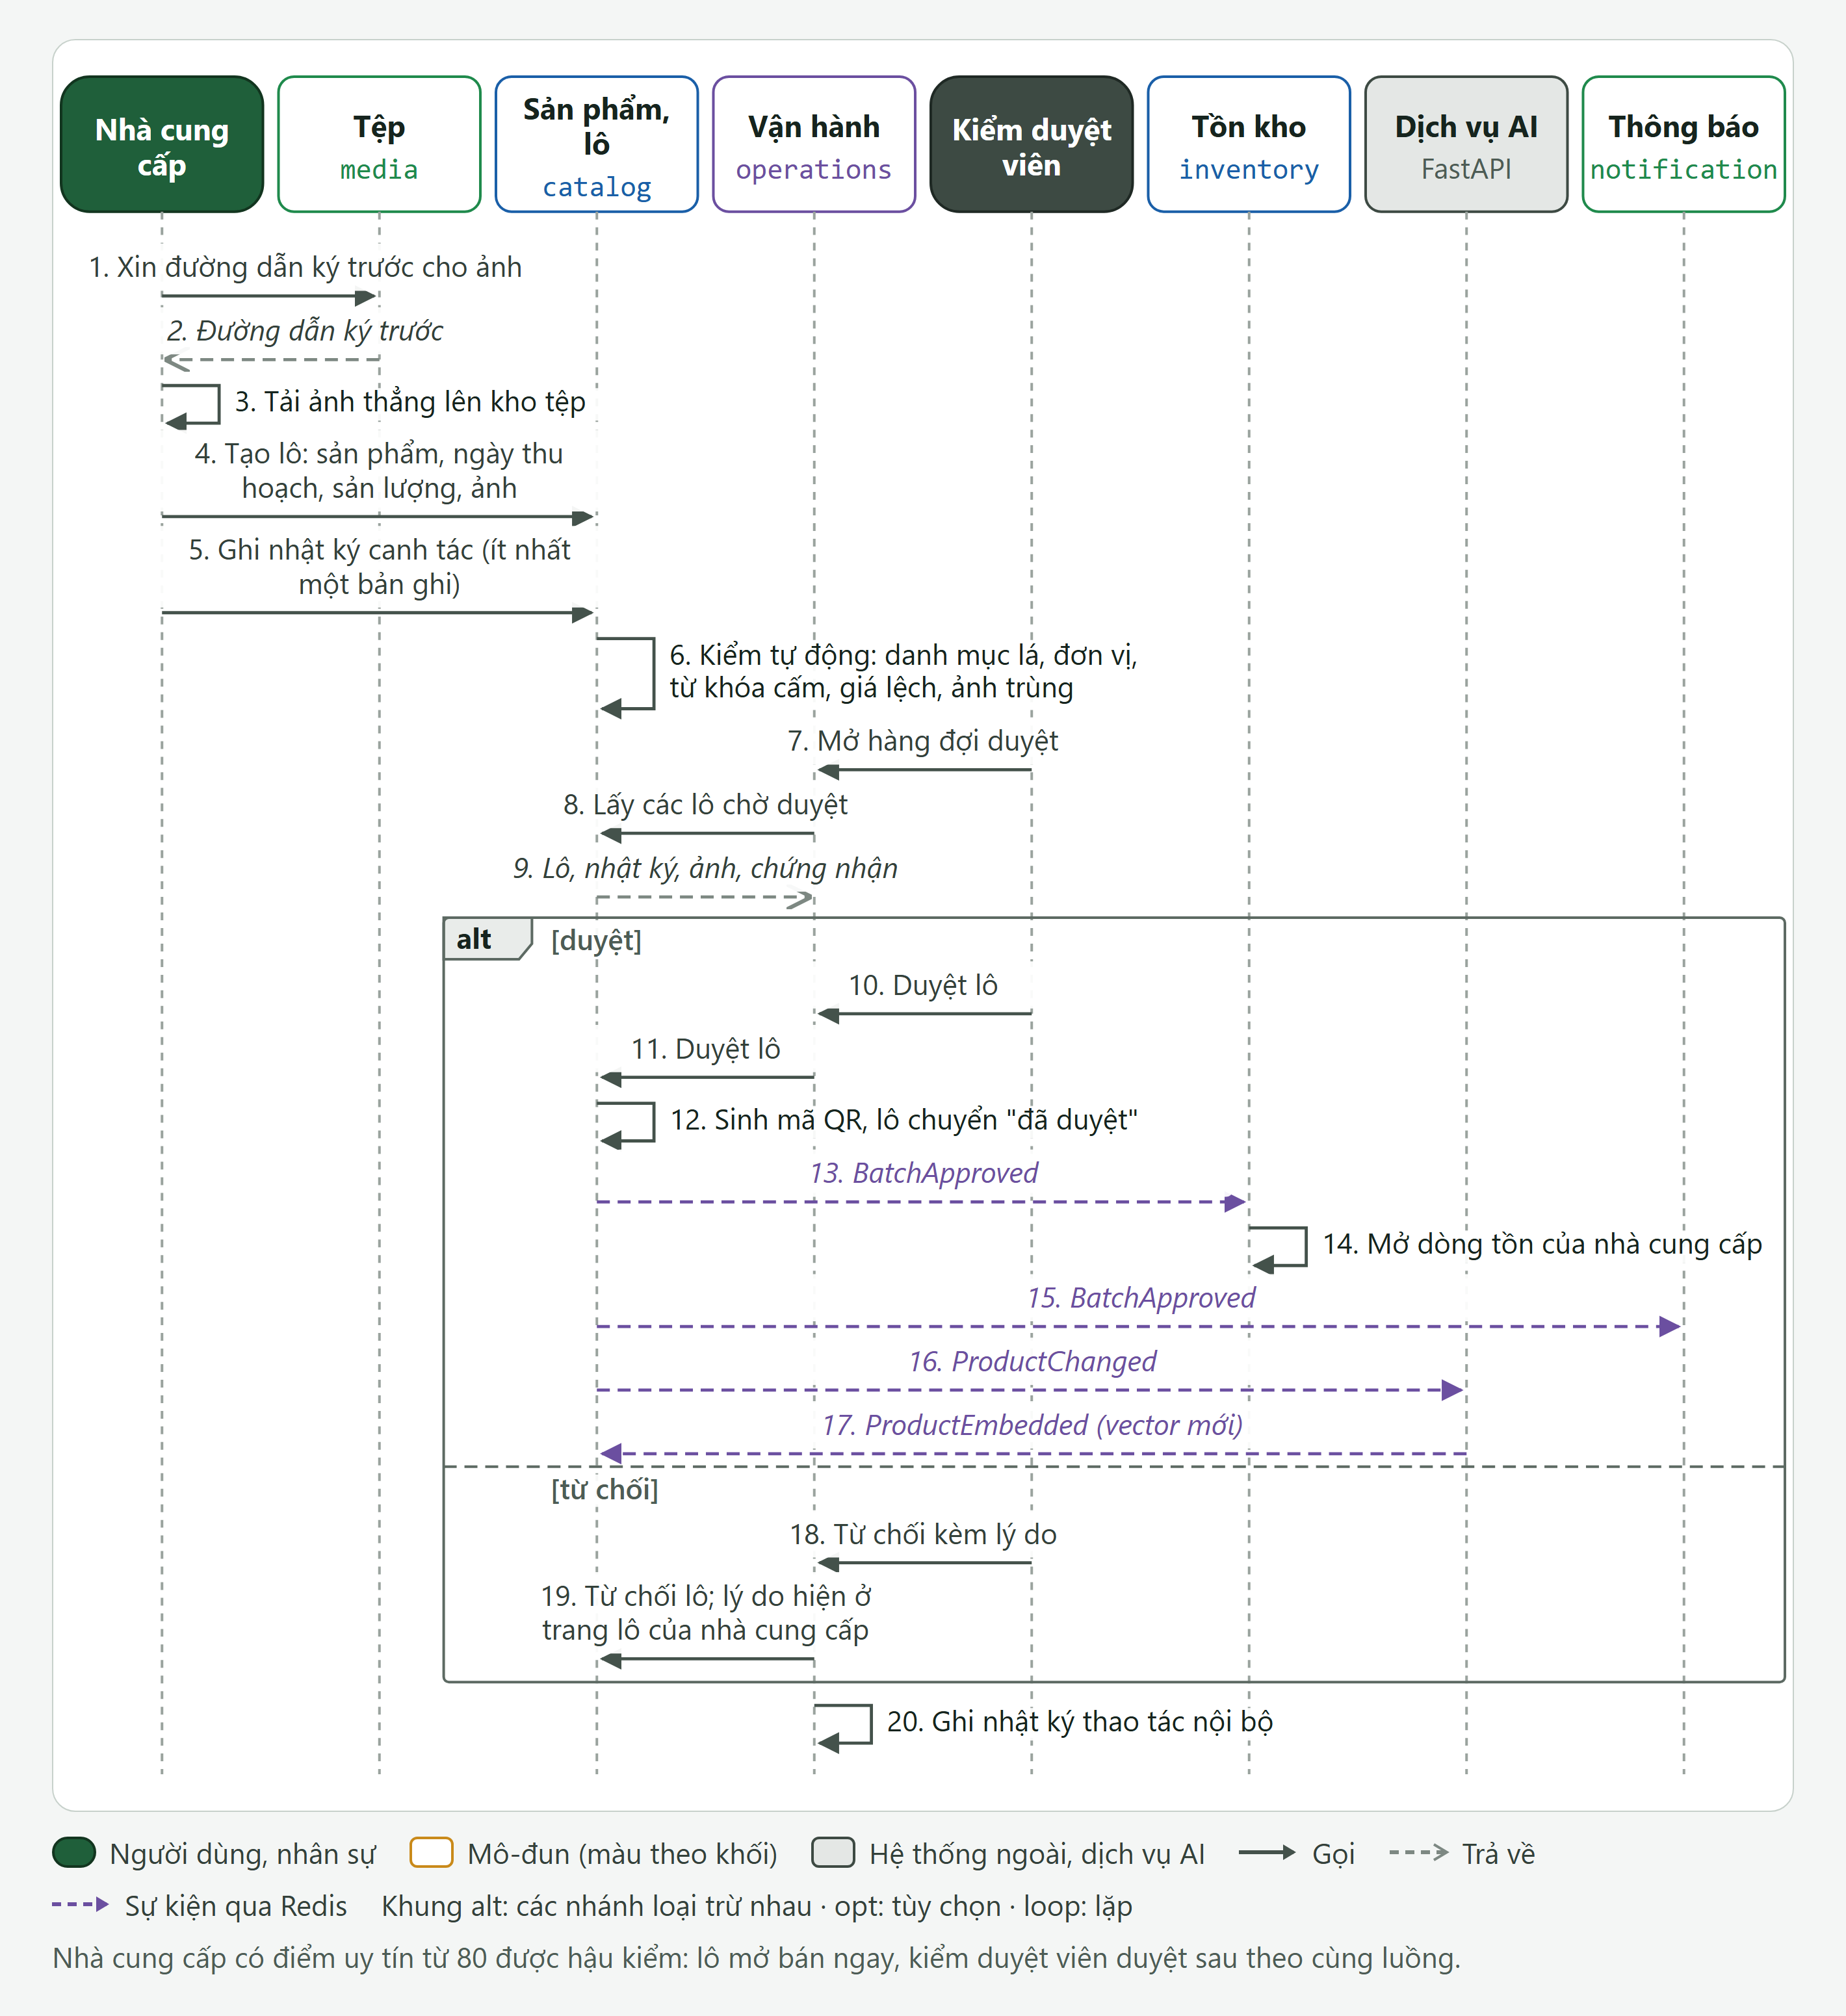
\includegraphics[width=\textwidth]{image/comparison/seq-duyet-lo.png}
\end{adjustbox}
\caption{Lược đồ tuần tự đăng lô, kiểm duyệt và sinh mã QR}
\label{fig:seq-duyet-lo}
\end{figure}

\begin{figure}[p]
\centering
\begin{adjustbox}{max totalsize={\textwidth}{\dimexpr\textheight-1.6cm\relax},center}
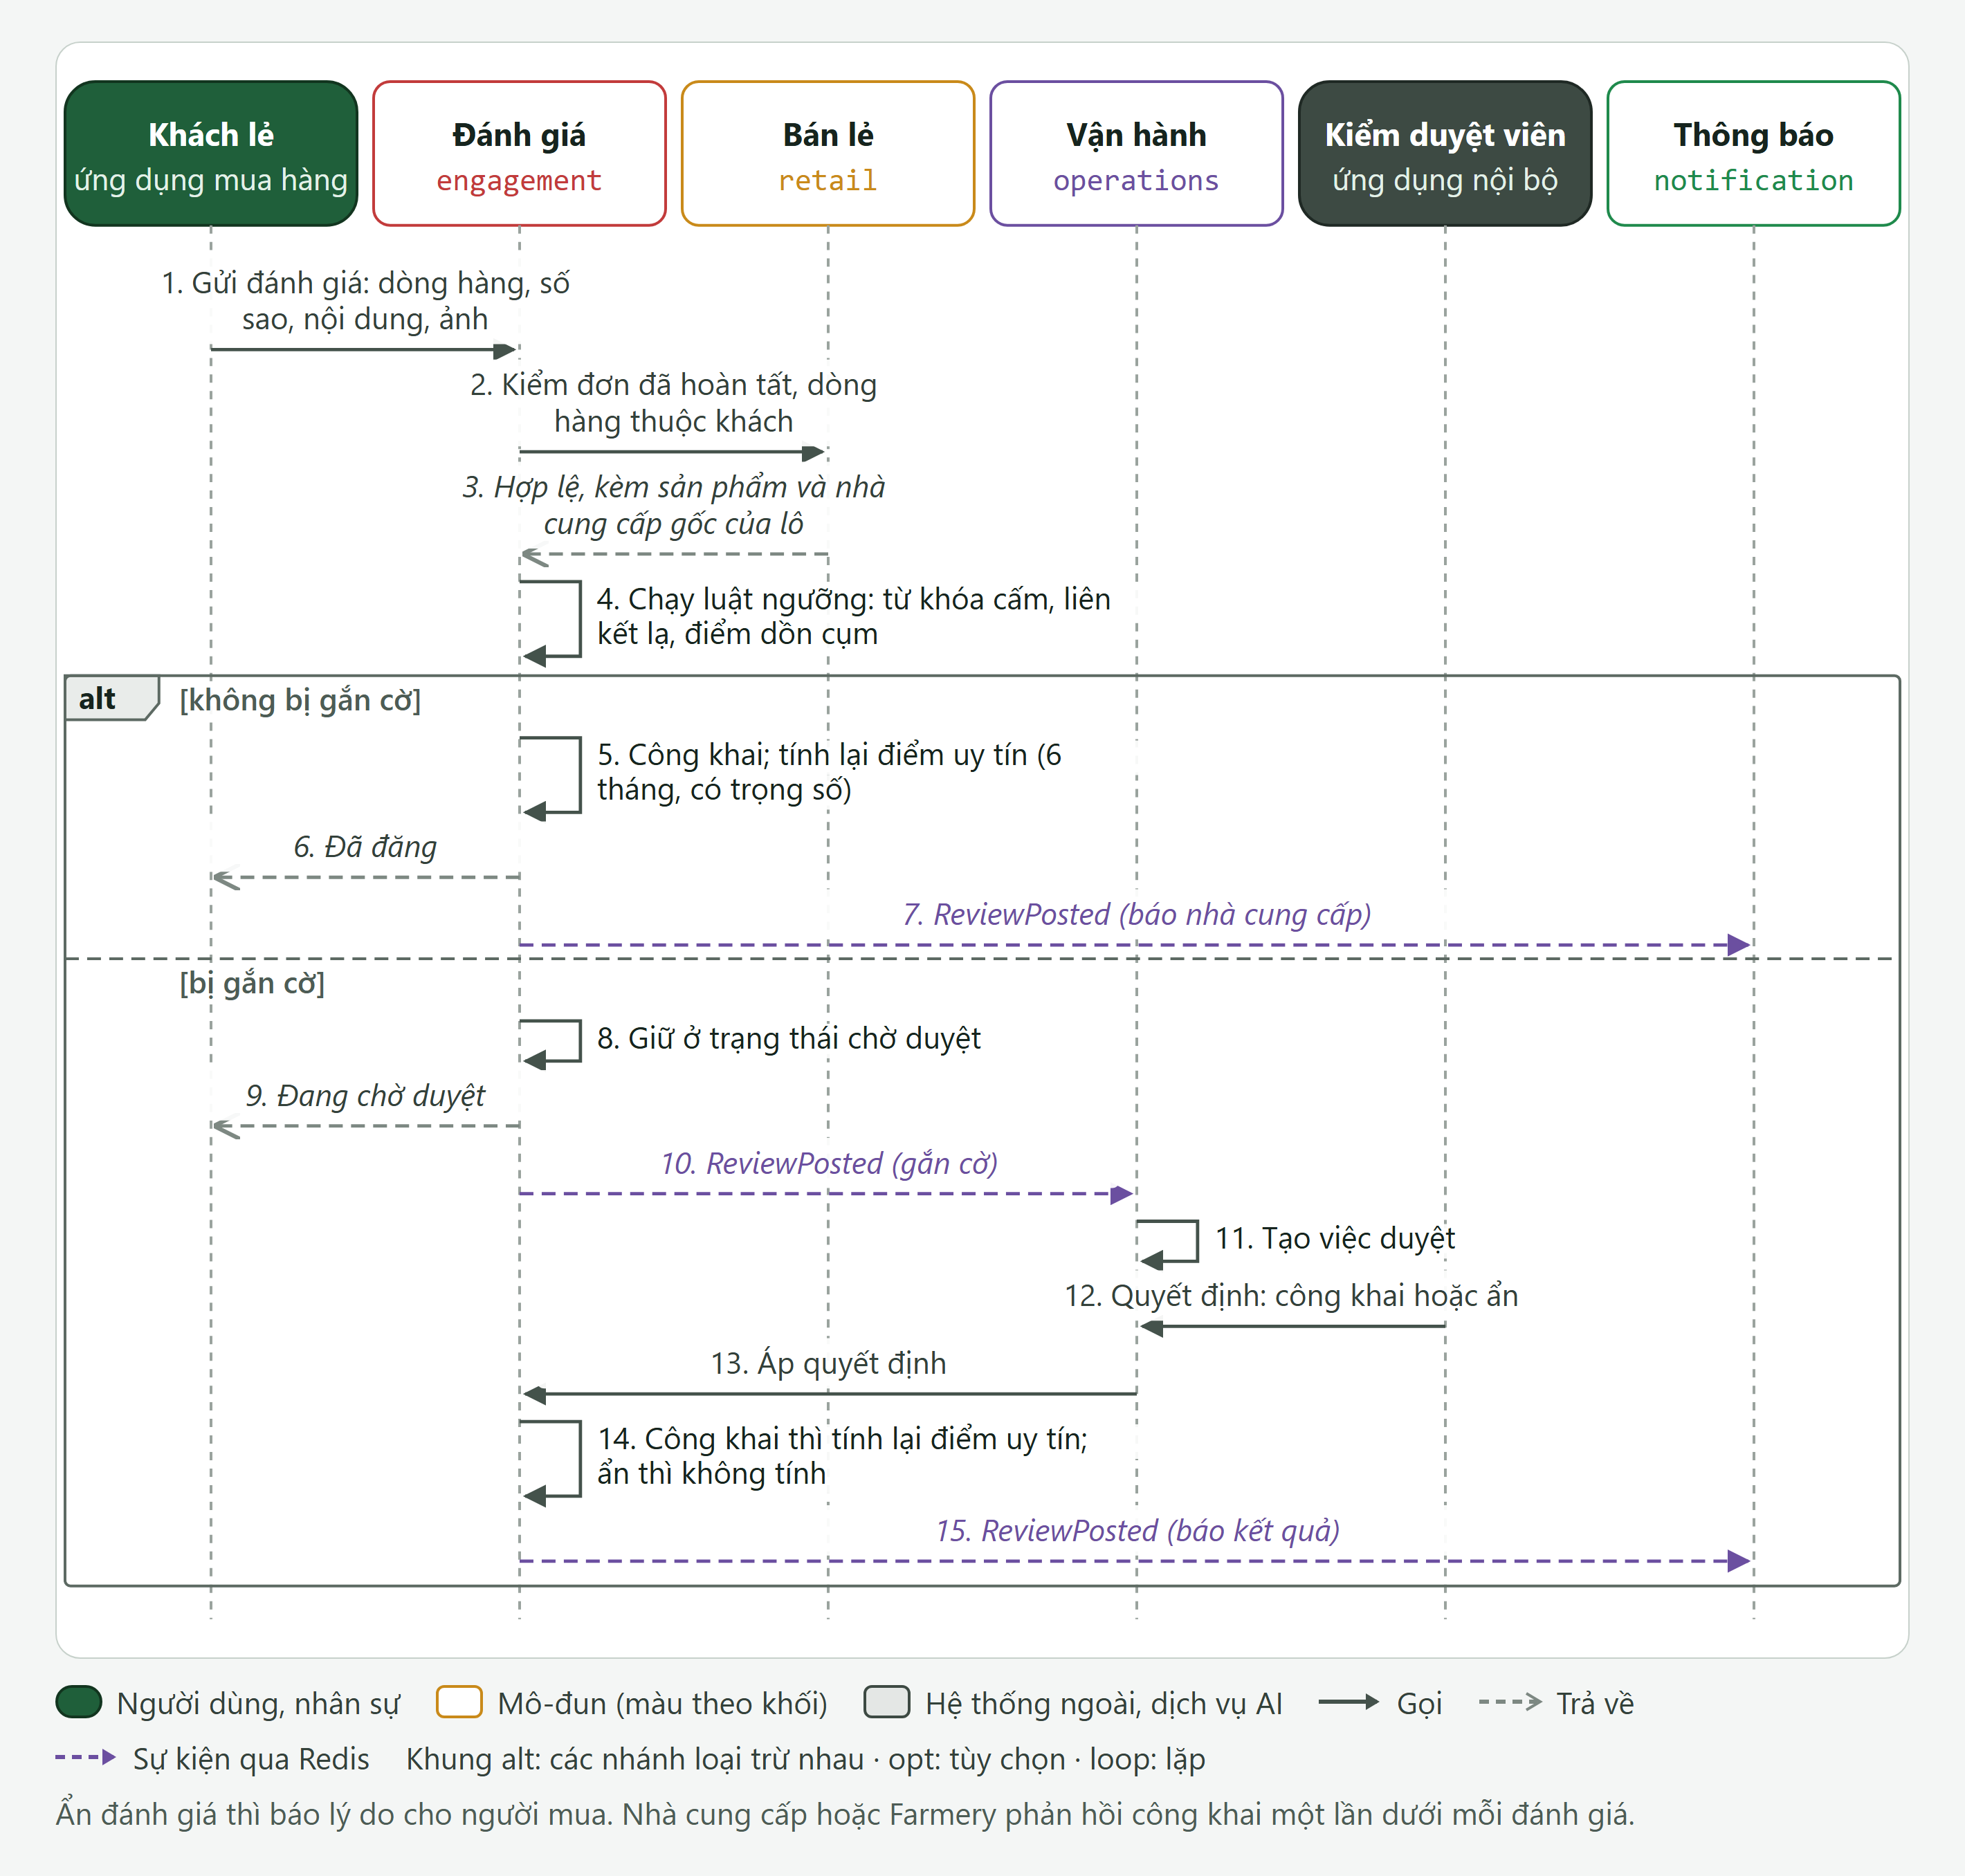
\includegraphics[width=\textwidth]{image/comparison/seq-danh-gia.png}
\end{adjustbox}
\caption{Lược đồ tuần tự gửi và kiểm duyệt đánh giá}
\label{fig:seq-danh-gia}
\end{figure}
